\vspace{-0.2cm}
\subsection{Theoretically Characterizing Implicit Regularization in TD-Learning}
\label{sec:theory} 
\vspace{-0.2cm}
Why does feature co-adaptation emerge in TD-learning and what do \emph{out-of-sample} actions have to do with it? To answer this question, we theoretically characterize the implicit regularization effects in TD-learning. We analyze the learning dynamics of TD learning in the overparameterized regime, where there are many different parameter vectors $\theta$ that fully minimize the training set temporal difference error. We base our analysis of TD learning on the analysis of implicit regularization in supervised learning, previously developed by \citet{blanc2020implicit,damian2021label}.

\textbf{Background.} When training an overparameterized $f_\theta(\bx)$ via supervised regression using the squared loss, denoted by $L$, many different values of $\theta$ will satisfy $L(\theta)=0$ on the training set due to overparameterization, but \citet{blanc2020implicit} show that the dynamics of stochastic gradient descent will only find fixed points $\theta^*$ that additionally satisfy a condition which can be expressed as $\nabla_\theta R(\theta^*) = 0$, along certain directions (that we will describe shortly). This function $R(\theta)$ is referred to as the implicit regularizer. The noisy gradient updates analyzed in this model have the form:  
\vspace{-0.05in}
\begin{equation}
\label{eq:gradient_update}
    \theta_{k+1} \leftarrow \theta_k - \eta \nabla_\theta L(\theta) + \eta \varepsilon_k, ~~ \varepsilon_k \sim \mathcal{N}(0, M).
\end{equation}
\vspace{-0.05in}
\citet{blanc2020implicit} and \citet{damian2021label} show that some common SGD techniques fall into this framework, for example, when the regression targets in supervised learning are corrupted with $\mathcal{N}(0, 1)$ label noise, then the resulting $M = \sum_{i=1}^{|\mathcal{D}|} \nabla_\theta f_\theta(\bx_i) \nabla_\theta f_\theta(\bx_i)^\top$ and the induced implicit regularizer $R$ is given by $R(\theta) = \sum_{i}^{|\mathcal{D}|} ||\nabla_\theta f_\theta(\bx_i)||_2^2$. Any solution $\theta^*$ found by Equation~\ref{eq:gradient_update} must satisfy $\nabla_\theta R(\theta^*) = 0$ along directions $\bv \in \mathbb{R}^{|\theta|}$ which lie in the null space of the Hessian of the loss $\nabla^2_\theta L(\theta^*)$ at $\theta^*$,  $\bv \in \text{Null}(\nabla^2_\theta L(\theta^*))$. The intuition behind the implicit regularization effect is that along such directions in the parameter space, the Hessian is unable to contract $\theta_k$ when running noisy gradient updates (Equation~\ref{eq:gradient_update}). Therefore, the only condition that the noisy gradient updates converge/stabilize at $\theta^*$ is given by the condition that $\nabla R(\theta^*) = 0$. This model corroborates empirical findings~\citep{mulayoff2020unique, damian2021label} about the solutions found by SGD, which motivates our use. 

\textbf{Our setup.} Following this framework, we analyze the fixed points of noisy TD-learning. We consider noisy pseudo-gradient (or semi-gradient) TD updates with a general noise covariance $M$:
\vspace{-0.05in}
\begin{align}
    \theta_{k+1} = \theta_k - \eta \underbrace{\left( \sum_i \nabla_\theta Q(\bs_i, \ba_i) \left(Q_\theta(\bs_i, \ba_i)\!- \!(r_i\!+\!\gamma {Q}_{\theta}(\bs'_i, \ba'_i))\right) \right)}_{:= g(\theta)} +\eta \varepsilon_k,  ~~ \varepsilon_k \sim \mathcal{N}(0, M)
\label{eq:td_update}
\end{align}
We use a deterministic policy $\ba'_i = \pi(\bs'_i)$ to simplify exposition. Following \citet{damian2021label}, we can set the noise model $M$ as $M = \sum_i \nabla_\theta Q(\bs_i, \ba_i) \nabla_\theta Q(\bs_i, \ba_i)^\top$, or utilize a different choice of $M$, but we will derive the general form first.  Let $\theta^*$ denote a stationary point of the training TD error, such that the pseudo-gradient
$g(\theta^*) = 0$. Further, we denote the derivative of $g(\theta)$ w.r.t. $\theta$ as the matrix $G(\theta) \in \mathbb{R}^{|\theta| \times |\theta|}$, and refer to it as the \emph{pseudo-Hessian}: although $G(\theta)$ is not actually the second derivative of any well-defined objective, since TD updates are not proper gradient updates, as we will see it will play a similar role to the Hessian in gradient descent. For brevity, define $G = G(\theta^*)$, $g = g(\theta^*)$, $\nabla G = \nabla_\theta G(\theta^*) \in \mathbb{R}^{|\theta| \times |\theta| \times |\theta|}$, and let $\lambda_i(P)$ denote the $i$-th eigenvalue of matrix $P$, when arranged in decreasing order of its (complex) magnitude $|\lambda_i(P)|$ (note that eigenvalues can be complex for non-symmetric matrices that we encounter here). 

\textbf{Assumptions.} To simplify analysis, we assume that matrices $G$ and $M$ (i.e., the noise covariance matrix) span the same $n$-dimensional basis in $d$-dimensional space, where $d$ is the number of parameters and $n$ is the number of datapoints, and $n \ll d$ due to overparameterization. We also require $\theta^*$ to satisfy a technical criterion that requires approximate alignment between the eigenspaces of $G$ and the gradient of the Q-function, without which noisy TD may not be stable at $\theta^*$. We summarize all the assumptions in Appendix~\ref{app:proofs}, and present the resulting regularizer below. 

\begin{theorem}[Implicit regularizer at TD fixed points]
\label{thm:implicit_noise_reg}
Under the assumptions so far, a fixed point of TD-learning,  $\theta^*$, where $Q_{\theta^*}(\bs_i, \ba_i) = r_i + \gamma Q_{\theta^*}(\bs'_i, \ba'_i)$ for every $(\bs_i, \ba_i, \bs'_i) \in \mathcal{D}$ is stable (atttractive) if: \textbf{(1)} it satisfies $\mathrm{Re}(\lambda_i(G)) \geq 0, \forall i$ and $\mathrm{Re}(\lambda_i(G)) > 0$ if $|\mathrm{Imag}(\lambda_i(G))| > 0$, and \textbf{(2)} along directions $\bv \in \mathbb{R}^{\text{dim}(\theta)}, \bv \in \text{Null}(G)$, $\theta^*$ is the stationary point of the implicit regularizer:
\vspace{-0.2cm}
\begin{align}
\label{eqn:regularizer}
R_\mathrm{TD}(\theta)\!\!&=\!\!\!\!\underbracket{\eta \sum_{i=1}^{|\mathcal{D}|} \nabla Q_\theta(\bs_i, \ba_i)^\top \Sigma^{*}_M \nabla Q_\theta(\bs_i, \ba_i)}_{\text{implicit regularizer for noisy GD in supervised learning}}
\!\!\!-\!\!\!\underbracket{\eta \gamma \sum_{i=1}^{|\mathcal{D}|} \mathrm{tr}\left(\left[\left[\nabla Q_\theta(\bs'_i, \ba'_i)^\top\right]\right]^\top \Sigma_M^* \nabla Q_\theta(\bs_i, \ba_i)  \right)}_{\text{additional term in TD learning}},
%%SL.10.27: would it be better to write the trace term as gradQ^T sigma gradQ (since tr(sigma gradQ gradQ^T) = tr(gradQ^T sigma gradQ))? that might make the similarity (but subtle difference) between the two terms more apparent...
    % R_\mathrm{TD}(\theta) = \sum_{i=1}^{|\mathcal{D}|} \mathrm{trace}\left[ \Sigma^{* \top}_M \nabla_\theta Q_\theta(\bs_i, \ba_i) \left( \nabla_\theta Q_\theta(\bs_i, \ba_i) - \gamma \texttt{Stop}(\nabla_\theta Q_\theta(\bs'_i, \ba'_i)) \right)^\top \right].  
    %%SL.9.29: I think it might be clearer if you write this as a difference of two terms, because then the first term will look like the supervised R(theta), but the second one will look clearly weird. The first term then becomes gradQ^T Sigma^T gradQ (and you don't need trace), which is very intuitive (also, Sigma is symmetric, right? so is the transpose symbol there necessary?). Additionally, consider using a less jarring symbol for Stop, so that the equation is typeset so that it looks more like -grad Q [gradQ^T] or something and the stop part is unobtrusive -- that would make it easier for readers to get intuition for what this equation means. Currently it's extremely hard to understand from looking at it.
\end{align}
% \vspace{-0.1in}
where $(\bs_i, \ba_i)$ and $(\bs'_i, \ba'_i)$ denote state-action pairs that appear together in a Bellman update, $[[\square]]$ denotes the stop-gradient function, which does not pass partial gradients w.r.t. $\theta$ into $\square$. $\Sigma^*_M$ is the fixed point of the  discrete Lyapunov equation: $\Sigma^*_M := (I - \eta G) \Sigma^*_M (I - \eta G)^\top + \eta^2 M$.
\end{theorem}
A proof of Theorem~\ref{thm:implicit_noise_reg} is provided in Appendix~\ref{app:proofs}. Next, we explain the intuition behind this result and provide a proof sketch. To derive the induced implicit regularizer for a stable fixed point $\theta^*$ of TD error, we study the learning dynamics of noisy TD learning (Equation~\ref{eq:td_update}) initialized at $\theta^*$, and derive conditions under which this noisy update would stay close to $\theta^*$ with multiple updates.  This gives rise to the two conditions shown in Theorem~\ref{thm:implicit_noise_reg} which can be understood as controlling stability in mutually exclusive directions in the parameter space. If condition \textbf{(1)} is not satisfied, then even under-parameterized TD will diverge away from $\theta^*$, since $I - \eta G$ would be a non-contraction as the spectral radius, $\rho(I - \eta G) \geq 1$ in that case. Thus, $\theta_k - \theta^*$ will grow or not decrease in some direction. When \textbf{(1)} is satisfied for all directions in the parameter space, there are still directions where both the real and imaginary parts of the eigenvalue $\lambda_i(G)$ are $0$ due to overparameterization\footnote{To see why this is the case, note that $\text{rank}(G) \leq |\mathcal{D}| \ll \text{dim}(\theta)$, and so some eigenvalues of $G$ are $0$.}. 
In such directions, learning is governed by the projection of the noise under the tensor  $\nabla G$,
%%SL.12.5: Are we making that mistake here again where we call the TD pseudo-gradient a derivative? I would recommend being *very* careful about the term derivative. Basically, don't call something a derivative if it's not really a derivative. You can introduce some term for it like pseudo-gradient, but it's very important to clearly distinguish between things that are actual derivatives or gradients, and the TD update. Try to avoid mixing the terminology, but it's OK to define some shorthand term like pseudo-gradient
%%AK: changed it here
which appears in the Taylor expansion of $\theta_k - \theta^*$ around the point $\theta^*$:
\begin{align}
    \label{eqn:nu_k}
    &\theta_{k+1} = \theta_k - \eta \left(g + G (\theta_k - \theta^*) + \frac{1}{2} \nabla G [\theta_k -\theta^*, \theta_k - \theta^*] \right) + \varepsilon_k, ~~ \varepsilon_k \sim \mathcal{N}(0, M)\\
    \implies &\nu_{k+1} = (I - \eta G )\nu_k  - \frac{\eta}{2} \nabla G [\nu_k, \nu_k] + \varepsilon_k,
    \label{eqn:nu_k_actual}
\end{align}
where we reparameterize in terms of $\nu_k := \theta_k - \theta^*$. The proof shows that $\theta^*$ is stable if it is a stationary point of the implicit regularizer $R_\mathrm{TD}$ (condition \textbf{(2)}), which ensures that total noise (i.e., accumulated $\varepsilon_k$ over iterations $k$) accumulated by $\nabla G$ does not lead to a large deviation in $\nu_k$ in directions where $I - \eta G$ does not contract. 
% The total noise accumulated with such noisy backups (Equation~\ref{eqn:nu_k}) admits the covariance matrix $\Sigma^*_M$, and the derivative of the regularizer $\nabla_\theta R_\mathrm{TD}(\theta)$ at an attractive $\theta^*$ must be zero to prevent any deviation in $\nu_k$ in directions where learning is controlled by \textbf{(2)}.   

% To derive the induced implicit regularizer for a stable fixed point $\theta^*$ of TD error, we study the learning dynamics of noisy TD learning (Equation~\ref{eq:td_update}) initialized at $\theta^*$, and derive conditions under which this noisy update would stay close to $\theta^*$ with multiple updates. In this case, we can utilize Taylor expansion around $\theta^*$ to track the evolution of the difference between $\theta_k$ and $\theta^*$, denoted as $\nu_k = \theta_k - \theta^*$ (roughly; modulo some terms we will discuss in Appendix~\ref{app:proofs}), as shown in Equation~\ref{eqn:nu_k}:
% \begin{align}
%     \label{eqn:nu_k}
%     &\theta_{k+1} = \theta_k - \eta \left(g + G (\theta_k - \theta^*) + \frac{1}{2} \nabla G [\theta_k -\theta^*, \theta_k - \theta^*] \right) + \varepsilon_k, ~~ \varepsilon_k \sim \mathcal{N}(0, M)\\
%     \implies &\nu_{k+1} = (I - \eta G )\nu_k  - \frac{\eta}{2} \nabla G [\nu_k, \nu_k] + \varepsilon_k.
%     \label{eqn:nu_k_actual}
% \end{align}
% Our theoretical result derives the implicit regularizer by characterizing conditions on $\theta^*$ that are necessary for the stability of the learning dynamics in Equation~\ref{eqn:nu_k_actual} in the neighborhood around $\theta^*$. 

\textbf{Interpretation of Theorem~\ref{thm:implicit_noise_reg}.} While the choice of the noise model $M$ will change the form of the implicit regularizer, in practice, the form of $M$ is not known as this corresponds to the noise induced via SGD. We can consider choices of $M$ for interpretation, but Theorem~\ref{thm:implicit_noise_reg} is easy to qualitatively interpret for $M$ such that $\Sigma^*_M = I$. In this case, we find that the implicit preference towards local minima of $R_\mathrm{TD}(\theta)$ can explain feature co-adaptation. In this case, the regularizer is simpler:
\begin{align*}
    R_\mathrm{TD}(\theta) := \sum_i ||\nabla Q_\theta(\bs_i, \ba_i) ||_2^2 - \gamma \nabla Q_\theta(\bs_i, \ba_i) \nabla [[Q_\theta(\bs'_i, \ba'_i)]].
\end{align*}
The first term is equal to the squared per-datapoint gradient norm, which is same as the implicit regularizer in supervised learning obtained by \citet{blanc2020implicit,damian2021label} with label noise. However, $R_\mathrm{TD}(\theta)$ additionally includes a second term that is equal to the dot product of the gradient of the Q-function at the current and next states, $\nabla_\theta Q_\theta(\bs_i, \ba_i)^\top \nabla_\theta Q_\theta(\bs'_i, \ba'_i)$, and thus this term is effectively \emph{maximized}. When restricted to the last-layer parameters of a neural network,
this term is equal to the dot product of the features at consecutive state-action tuples: $\sum_i \nabla_\theta Q_\theta(\bs_i, \ba_i)^\top \nabla_\theta Q_\theta (\bs'_i, \ba'_i) = \sum_i \phi(\bs_i, \ba_i)^\top \phi(\bs'_i, \ba'_i)$. The tendency to maximize this quantity to attain a local minimizer of the implicit regularizer corroborates the empirical findings of increased dot product in Section~\ref{app:problem_more}. 

\textbf{Explaining the difference between utilizing seen and unseen actions in the backup.} If all state-action pairs $(\bs'_i, \ba'_i)$ appearing on the right-hand-side of the Bellman update also appear in the dataset $\mathcal{D}$, as in the case of offline SARSA (Figure~\ref{fig:dot_products}), the preference to increase dot products will be balanced by the affinity to reduce gradient norm (first term of $R_\mathrm{TD}(\theta)$ when $\Sigma^*_M = I$): for example, for offline SARSA, when $(\bs'_i, \ba'_i)$ are permutations of $(\bs_i, \ba_i)$, $R_\mathrm{TD}$ is lower bounded by $(1 - \gamma) \sum_i ||\nabla_\theta Q_\theta(\bx_i)||_2^2$ and hence minimizing $R_\mathrm{TD}(\theta)$ would minimize the feature norm instead of maximizing dot products. This also corresponds to the implicit regularizer we would obtain when training Q-functions via supervised learning and hence, our analysis predicts that offline SARSA with in-sample actions (i.e., when $(\bs', \ba') \in \mathcal{D}$) would behave similarly to supervised regression. 

However, the regularizer behaves very differently when unseen state-action pairs $(\bs'_i, \ba'_i)$ appear only on the right-hand-side of the backup. This happens with any algorithm where $\ba'$ is not the dataset action, which is the case for all deep RL algorithms that compute target values by selecting $\ba'$ according to the current policy. In this case, we expect the dot product of gradients at $(\bs, \ba)$ and $(\bs', \ba')$ to be large at any attractive fixed point, since this minimizes $R_\mathrm{TD}(\theta)$. This is precisely a form of co-adaptation: \textit{gradients at out-of-sample state-action tuples are highly similar to gradients at observed state-action pairs measured by the dot product}. This observation is also supported by the analysis in Section~\ref{app:problem_more}. Finally, note that the choice of $M$ is a modelling assumption, and to derive our explicit regularizer, later in the paper, we will make a simplifying choice of $M$. However, we also empirically verify that a different choice of $M$, given by label noise, works well.
%%%%%%%%%%%%%%%%%%%%%%%%%%%%%%%%%%%%%%%%%%%%%%%%%%%%%%%%%%


\begin{figure}[t]
    \centering
    % \vspace{-18pt}
    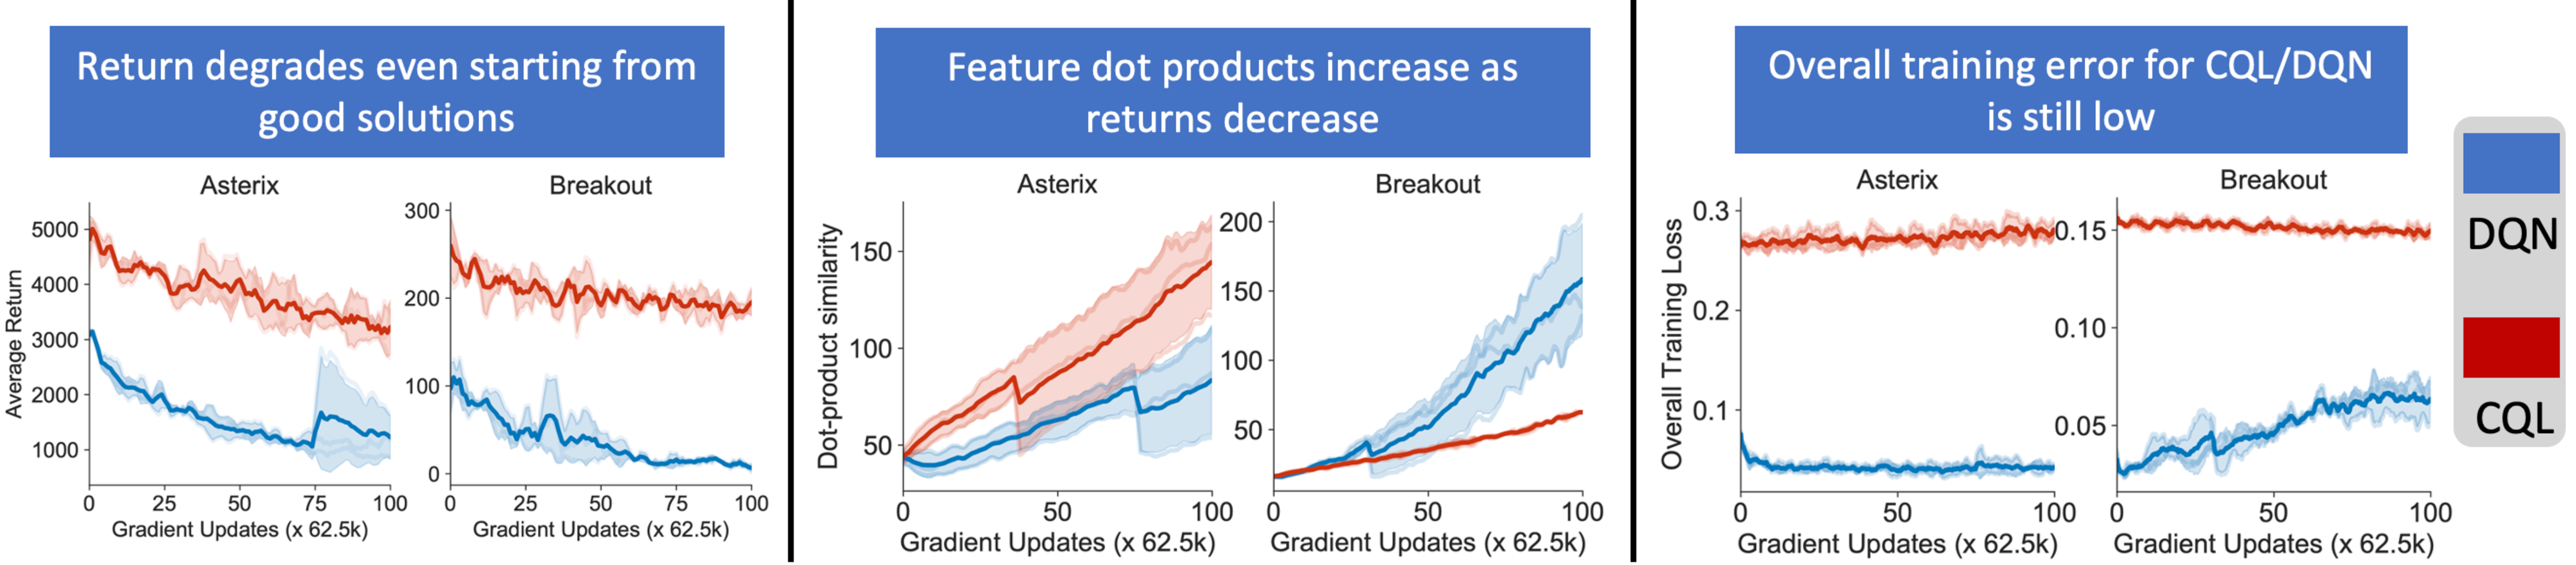
\includegraphics[width=0.99\linewidth]{figures_iclr/return_degrades.pdf}
    % 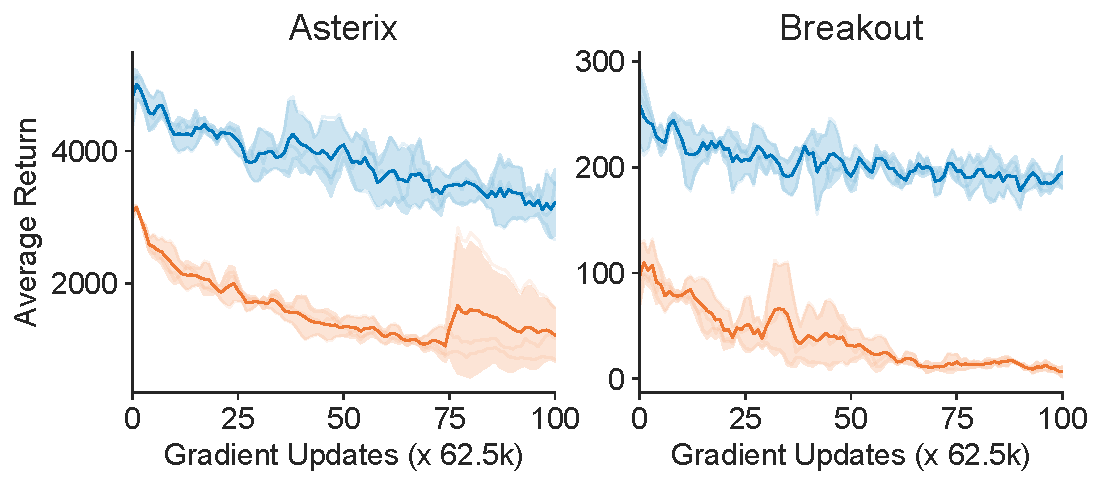
\includegraphics[width=0.49\linewidth]{figures/figure3_neurips_stability_cql_dot_product_both_return.pdf}
    \vspace{-0.3cm}
    \caption{\small{Even when current offline RL algorithms are initialized at a high-performing checkpoint that attains small feature dot products, feature dot products increase with further training and the performance degrades.}}  
    %%SL.7.13: I don't really understand the implication of the last part ("note that the values of the TD error and the overall training loss for either algorithm are generally low and decrease in many cases")
    \label{fig:stability}
    \vspace{-0.55cm}
\end{figure}



\textbf{Why is implicit regularization detrimental to policy performance?}
To answer this question, we present theoretical and empirical evidence that illustrates the adverse effects of this implicit regularizer. Empirically, we ran two algorithms, DQN and CQL, initialized from a high-performing Q-function checkpoint,
%%SL.10.27: This part is going to really throw off some readers. Of course it's not a stable point for TD, because you didn't learn it with TD! Why do we expect the solution found by one method (in this case DR3) to be stable for another method? That doesn't illustrate that TD is bad, just that DR3 changes the fixed point (which it should). But perhaps if you don't want to go into detail about this issue, you could somehow sweep the "obtained using DR3" bit under the rug to avoid distracting the reader?
%%AK: agreed, removed
which attains relatively small feature dot products (i.e., the second term of $R_\mathrm{TD}(\theta)$ is small). Our goal is to see if TD updates starting from such a ``good'' initialization still stay around it or diverge to poorer solutions. Our theoretical analysis in Section~\ref{sec:theory} would predict that TD learning would destabilize from such a solution, since it would not be a stable fixed point. Indeed, as shown in Figure~\ref{fig:stability}, the policy immediately degrades, and the the dot-product similarities start to increase. This even happens with CQL, which explicitly corrects for distributional shift confounds, implying that the performance drop cannot be directly explained by the typical out-of-distribution action explanations. To investigate the reasons behind this drop, we also measured the training loss function values for these algorithms (i.e., TD error for DQN and TD error + CQL regularizer for CQL) and find in Figure~\ref{fig:stability} that the loss values are generally small for both CQL and DQN. This indicates that the preference to increase dot products is not explained by an inability to minimize TD error. 
%%SL.12.5: I don't understand what "implicit phenomenon" means or how the loss being low indicates this
In Appendix~\ref{app:cql_stability}, we show that this drop in performance when starting from good solutions can be effectively mitigated with our proposed \methodname\ explicit regularizer for both DQN and CQL. Thus we find that not only standard TD learning degrades from a good solution in favor of increasing feature dot products, but keeping small dot products enables these algorithms to remain stable near the good solution.
%%SL.12.5: I slightly tweaked the above sentence, but it can be badly misunderstood as saying that basically our entire evaluation of DR3 has been offloaded into that appendix.

To motivate why co-adapted features can lead to poor performance in TD-learning, we study the convergence of linear TD-learning on co-adapted features. Our theoretical result characterizes a lower bound on the feature dot products in terms of the feature norms for state-action pairs in the dataset $\mathcal{D}$, which if satisfied, will inhibit  convergence: 
\begin{proposition}[TD-learning on co-adapted features]
\label{thm:co_adapted_features_are_bad}
Assume that the features $\Phi = [\phi(\bs, \ba)]_{\bs, \ba}$ are used for linear TD-learning. Then, if $\sum_{\bs, \ba, \bs' \in \mathcal{D}} \phi(\bs, \ba)^\top \phi(\bs', \ba') \geq \frac{1}{\gamma} \sum_{\bs, \ba \in \mathcal{D}} \phi(\bs, \ba)^\top \phi(\bs, \ba)$, linear TD-learning using features $\Phi$ will not converge. 
\end{proposition}
A proof of Proposition~\ref{thm:co_adapted_features_are_bad} is provided in Appendix~\ref{app:new_thm} and it relies on a stability analysis of linear TD. While features change during training for TD-learning with neural networks, and arguably linear TD is a simple model to study consequences of co-adapted features, even in this simple linear setting, Proposition~\ref{thm:co_adapted_features_are_bad} indicates that TD-learning may be non-convergent as a result of co-adaptation.

% \textbf{Comparison to implicit regularization in TD learning with linear function approximation.} Running stochastic gradient descent in overparameterized linear regression finds solutions with the smallest $\ell_2$ norm, which is often regarded as the implicit regularizer. Based on this observation, one might wonder how our derived implicit regularizer relates to minimum norm solutions attained by gradient descent in overparameterized linear TD learning. The implicit regularizer we obtain in  Equation~\ref{eqn:regularizer} would be a constant, independent of the parameter vector $\theta$ for linear TD learning. Thus our regularization specifically captures the effect of SGD on non-linear function approximators, which are absent when studying linear function approximation. 

% \textbf{Takeaways.} We summarize the key takeaways from our theoretical analysis now. \textbf{(1)} \emph{The implicit regularizer at TD fixed points} is shown in Equation~\ref{eqn:regularizer}. The first term corresponds to the regularizer for SGD in supervised learning, while the second term that is unique to TD and leads to an (undesirable) increase in gradient or feature dot products; \textbf{(2)}\emph{Out-of-sample actions exacerbate the implicit regularization effect,} since feature dot products can be easily increased when out-of-sample actions, which do not appear in the dataset, are used to compute Bellman targets; \textbf{(3)} The implicit regularizer in Equation~\ref{eqn:regularizer} is induced via a mechanism unique to non-linear Q-functions, different from overparameterized, linear TD-learning.
% \vspace{-0.15cm}

% \textbf{Theoretically,} we characterize the adverse effects of this implicit regularization by examining the trend in the worst-case error incurred by value-function learning on top of the learned features as feature dot-products increase.